
Let $\vec{p} = \myvec{1\\2\\3}$ be a point on the line L.
Direction vector of the  line perpendicular to the given plane is
\begin{align}
 \myvec{1\\2\\-5}
\end{align}
Thus, the equation of required line is
\begin{align}
    L: \quad \vec{x}&=\vec{p}+\lambda\vec{a}\\ &=\myvec{1\\2\\3}+\lambda\myvec{1\\2\\-5}
\end{align}
See Fig.  \ref{aug/2/34/plot}.
\begin{figure}[!h]
 \centering
 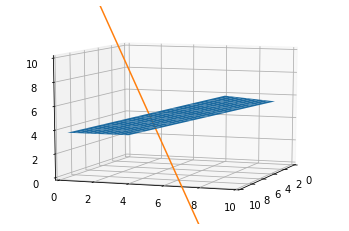
\includegraphics[width=\columnwidth]{solutions/aug/2/34/figs/Assignment4.png}
 \caption{Plot of plane and the line}
 \label{aug/2/34/plot}
\end{figure}


